\documentclass[conference]{IEEEtran}
\IEEEoverridecommandlockouts
% The preceding line is only needed to identify funding in the first footnote. If that is unneeded, please comment it out.
\usepackage{cite}
\usepackage{amsmath,amssymb,amsfonts}
\usepackage{algorithmic}
\usepackage{graphicx}
\usepackage{textcomp}
\usepackage{xcolor}
\def\BibTeX{{\rm B\kern-.05em{\sc i\kern-.025em b}\kern-.08em
    T\kern-.1667em\lower.7ex\hbox{E}\kern-.125emX}}
\begin{document}

\title{Privacy-Preserving Face Recognition in the Frequency Domain\\
%{\footnotesize \textsuperscript{*}Note: Sub-titles are not captured in Xplore and should not be used}
%\thanks{Identify applicable funding agency here. If none, delete this.}
}

\author{\IEEEauthorblockN{Xiyang Hu}
\IEEEauthorblockA{\textit{Computer Science \& Engineering} \\
\textit{Lehigh University}\\
%Bethlehem, USA \\
xih322@lehigh.edu}
\and
\IEEEauthorblockN{Zhikai Wang}
\IEEEauthorblockA{\textit{Computer Science \& Engineering} \\
\textit{Lehigh University}\\
%Bethlehem, USA \\
zhw622@lehigh.edu}
\and
\IEEEauthorblockN{Jiageng Zheng}
\IEEEauthorblockA{\textit{Computer Science \& Engineering} \\
\textit{Lehigh University}\\
%Bethlehem, USA \\
jiz322@lehigh.edu}

}

\maketitle

%\begin{abstract}
%This document is a model and instructions for \LaTeX.
%This and the IEEEtran.cls file define the components of your paper [title, text, heads, etc.]. *CRITICAL: Do Not Use Symbols, Special Characters, Footnotes, 
%or Math in Paper Title or Abstract.
%\end{abstract}

%\begin{IEEEkeywords}
%component, formatting, style, styling, insert
%\end{IEEEkeywords}

\section{Introduction}
With the rapid development of deep learning, the protection of user privacy has become crucial for most applications. Especially in the process of facial recognition, no parties should disclose user's privacy of any type. However, as more attacking methods are discovered and explored, we have to be aware of all possible risks which may threaten users' security and privacy when designing a machine learning system. Attackers can easily insert their triggers into the training data to threaten user's security, such as [1], [2], [3]. Moreover, attackers can predict the existence of a person in the training dataset, threatening users' privacy. \\ \indent
Based on [4], [5], we implement a privacy-preserved face recognition to solve the privacy concerns. We use the discrete cosine transform (DCT) to convert the images to frequency domain, because DCT separates information critical to visualization from information critical to identification. Next, we add noises to the model training process to preserve the privacy. By using concepts from differential privacy, we quantify the privacy protection. The model will be evaluated based on both privacy protection and its accuracy.

\section{Project Type and our Contribution}
We develop neural network architectures for the datasets we selected, train the model for a decent accuracy, and then implement algorithms for privacy-preserving, which achieves a fast inference time and satisfactory trade-off between privacy and accuracy. (ideally) 

\section{Methodology}
\subsection{Convolutional Neural Network}\label{AA}
The Convolutional Neural Network (CNN) is commonly used in image recognition tasks. 
In contrast to the fully connected layers, the convolutional layers
in CNN allow the model to encode image-specific features. As a result, the model is
more suited for image classification tasks  \cite{b6}. Moreover, the convolutional layers typically require fewer trainable parameters than fully connected layers, which makes the resulting model smaller in size.

\subsection{Activation Function}
Different than linear classifiers, any neural network model needs activation function to achieve non-linearity. 
Typical activation function includes sigmoid, tanh, and Relu. For the last neural network layer, softmax activation are commonly used to map an output vector to possibilities of each class. For intermediate layers, the Relu activation and its variants are commonly used because they are easy to compute and they does not have gradient vanishing problem \cite{b7}.

\subsection{Batch Normalization}
The optimization process of neural network training updates trainable parameters, and as a result, the distributions of layers' input will be constantly changed. The method of batch normalization is proposed \cite{b8}. They normalize the input for each layers within each mini-batches, and scale and shift the result based on two trainable parameters. By considering batch normalization as a part of neural network architecture, the neural network model can reach a decent accuracy with less training epochs.

\subsection{Data Augmentation}
For many tasks, the amount of data is not sufficient to train a model without overfitting. Data augmentation techniques can be used to increase the size of training data. It contributes to the learning system by increasing testing accuracy and the robustness of the model. There are various data augmentation techniques. For example, geometric transformations, color space augmentations, kernel filters, mixing images, random erasing, feature space augmentation, adversarial training, generative adversarial networks, neural style transfer, and meta-learning \cite{b9}. For our task, we will use the most basic ways (i.e. random crop) to augment the face images.

\subsection{Transformers}
The models using Transformers architecture has recently reached state-of-art accuracy for tasks in computer vision. Works have shown that the ideas from transformers can help to achieve the 99.5 percent testing accuracy on CIFAR-10 without using convolutional layers \cite{b10}. If we have sufficient time, we will explore the feasibility of transformer models for this project.

\subsection{Data Transformation}
The spatial domain contains the pixels of the image, and each pixels can be manipulated directly. There are two common color spaces used to record or display color images, RGB and YUV. RGB is the combination of red, green, and blue light. YUV is the combination of luminance, blue projection chrominance, and red projection chrominance. Since the YUV is closer to human vision than RGB and has better perceptual quality [11], YUV is increasingly used in the field of image processing [12].
The frequency domain is a new perspective of image processing. In the frequency domain, the high-frequency represent the edges of the image, and the low-frequency represent the smooth regions in the image. The transformation from spatial domain to frequency domain is Fourier transform. DFT (Discrete Fourier Transform), DCT (Discrete Cosine Transform), and DWT (Discrete Wavelet Transform) are the most classical transform methods. DCT and DWT is developed from DFT and is widely used in image processing due to the better performance. 

\subsection{Data Perturbation}
For face recognization systems, the best way to preserve privacy of data provider is to not collect their facial image. Instead, parties that train the model can collect images after random perturbation. However, training with perturbed data may decrease the prediction accuracy. In this project, we intend to explore the feasibility of pre-training privacy preservation on different datasets for different classification tasks.

\subsection{Membership Inference Attack}
Imagine a company that trained a neural network model which takes a face image and outputs the possibility distribution for the age of the face. If this company provides the trained model as a service, the privacy of data providers is leaked. By analyzing the model outputs, malicious users can predict whether a person is a part of the training set \cite{b13}. For example, having a smaller entropy in the output distribution indicate the input is more likely included in the training set. To infer the membership of a person with respect to the training set, the attacker can also leverage model output using deep learning techniques.

\subsection{Output Perturbation and Differential Privacy}
To protect the data provider's privacy against the Membership Inference Attack, the service provider can add random noise to the output vector. The service provider can also perturb the gradients during training \cite{b14}. Depending on the magnitude of the noise, the service provider can use differential privacy concepts to quantify the privacy preservation and report it to data providers.

\section{Network Architecture (Current)}
Until the midterm, we have designed a simple network architecture (also submitted with code). It uses convectional layers, Relu activations, max pooling, linear layers, and a softmax layer (fig. 1.).  Notice that the input has only 1 dimension because inputs are grayscale images. We will later refine this architecture and expand this to color images.
\begin{figure}[htbp]
\centerline{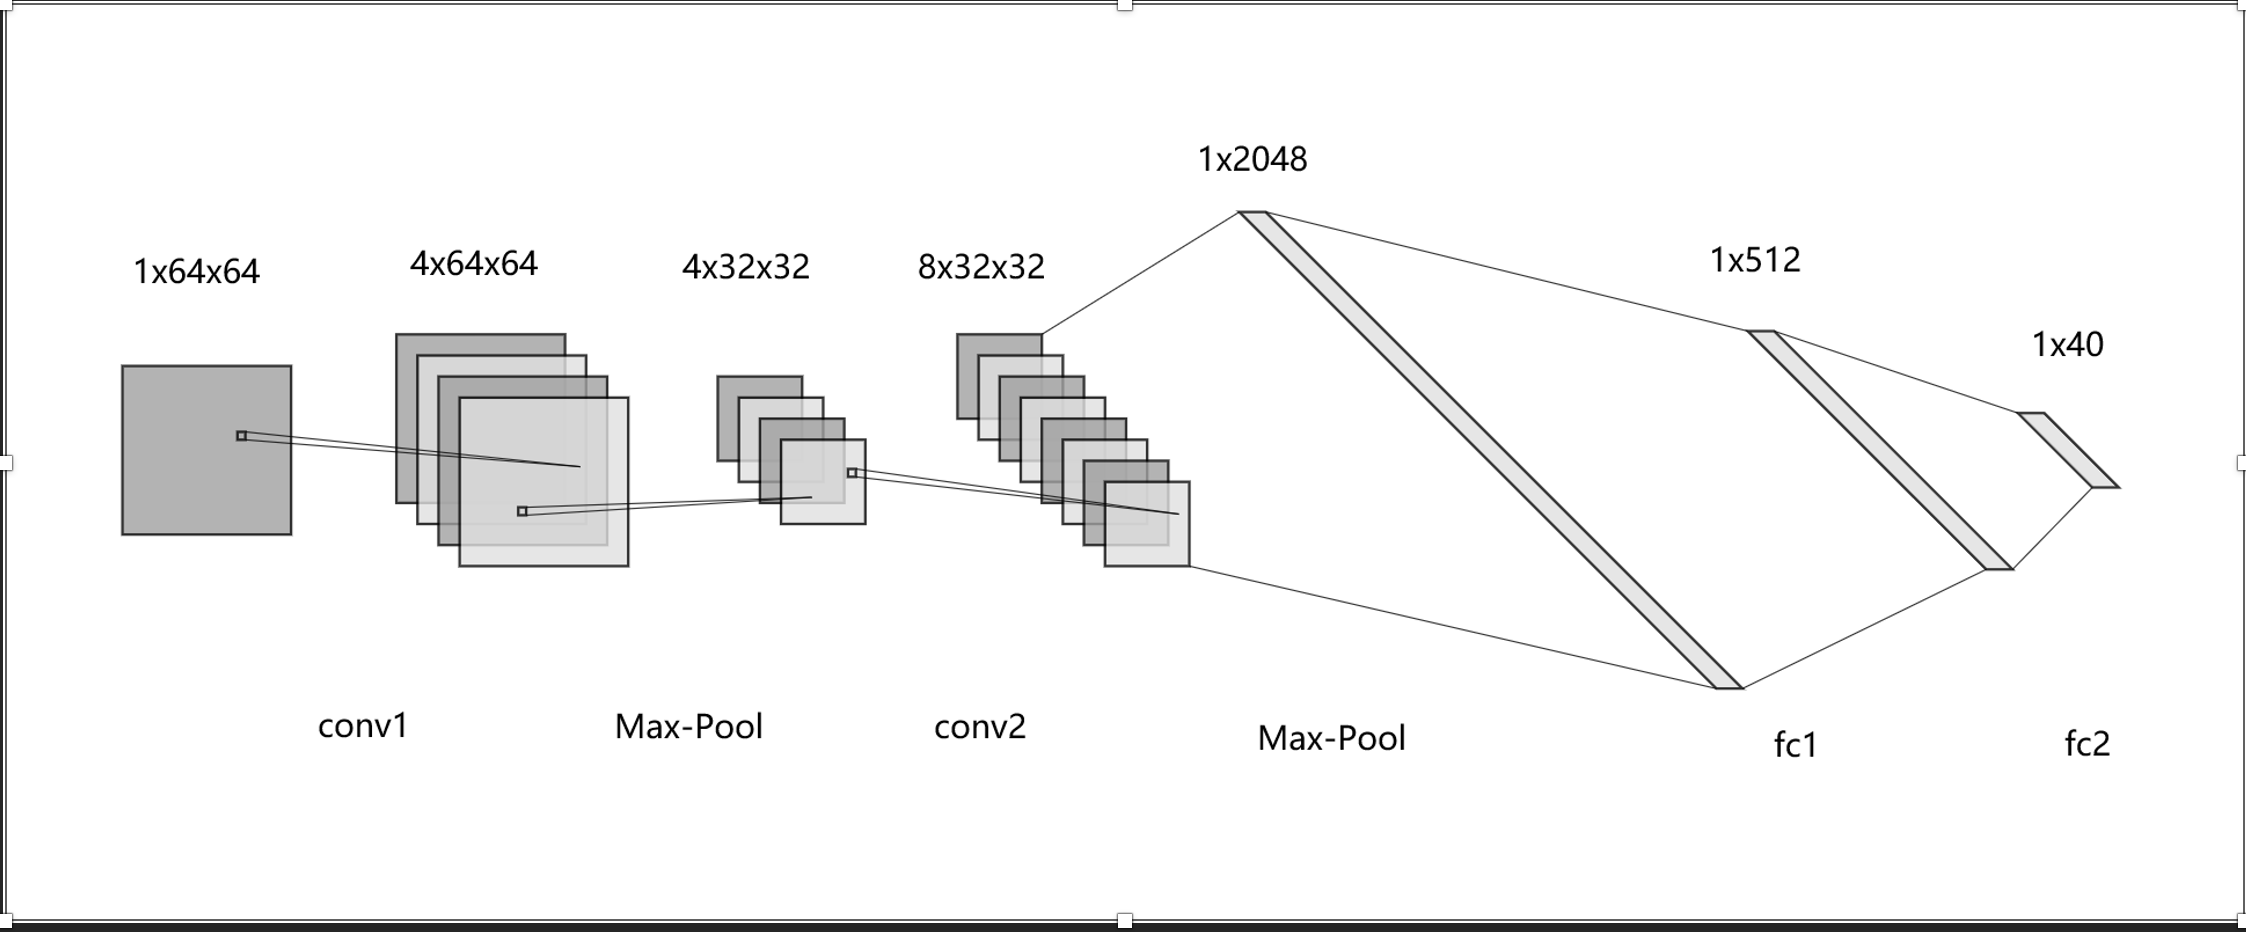
\includegraphics[width=80mm]{architecture.png}}
\caption{Simple nn architecture we have implemented, kernel size 3*3 with padding 1}
\label{fig}
\end{figure}

\begin{thebibliography}{00}


\bibitem{b1} Yue, Chang, et al, ``Invisible Backdoor Attacks Using Data Poisoning in the Frequency Domain,''  arXiv preprint arXiv:2207.04209 2022
\bibitem{b2} Tianyu Gu, Kang Liu, Brendan Dolan-Gavitt, Siddharth Garg, ``Badnets: Evaluating Backdooring Attacks on Deep Neural Networks,'' IEEE Access, 7:47230– 47244, 2019
\bibitem{b3} Xinyun Chen, Chang Liu, Bo Li, Kimberly Lu, Dawn Xiaodong Song, ``Targeted backdoor attacks on deep learning systems using data poisoning,'' ArXiv, abs/1712.05526, 2017
\bibitem{b4}  Wang, Yinggui, et al.  `Privacy-Preserving Face Recognition in the Frequency Domain,''  2022
\bibitem{b5} Ji, Jiazhen, et al, ``Privacy-Preserving Face Recognition with Learnable Privacy Budgets in Frequency Domain,''  	arXiv preprint arXiv:2207.07316 2022
\bibitem{b6} Keiron O’Shea, Ryan Nash, ``An Introduction to Convolutional Neural Networks,'' arXiv:1511.08458v2, 2015
\bibitem{b7} Siddharth Sharma, Simone Sharma, Anidhya Athaiya, ``ACTIVATION FUNCTIONS IN NEURAL NETWORKS'', International Journal of Engineering Applied Sciences and Technology, 2020
Vol. 4, Issue 12, ISSN No. 2455-2143, Pages 310-316 
\bibitem{b8} Sergey Ioffe, Christian Szegedy, ``Batch Normalization: Accelerating Deep Network Training by Reducing Internal Covariate Shift,''  arXiv:1502.03167, 2015
\bibitem{b9} Connor Shorten, Taghi M. Khoshgoftaar, ``A survey on Image Data Augmentation for Deep Learning,'' Shorten and Khoshgoftaar J Big Data 2019
\bibitem{b10} Alexey Dosovitskiy, Lucas Beyer, Alexander Kolesnikov, Dirk Weissenborn, Xiaohua Zhai, Thomas Unterthiner, Mostafa Dehghani, Matthias Minderer, Georg Heigold, Sylvain Gelly, Jakob Uszkoreit, Neil Houlsby, ``AN IMAGE IS WORTH 16X16 WORDS: TRANSFORMERS FOR IMAGE RECOGNITION AT SCALE,'' ICLR 2021

\bibitem{b11} Michal Podpora, Grzegorz Pawel Korbas, Aleksandra Kawala-Janik, `` Yuv vs rgb-choosing a color space for human-machine interaction,''  FedCSIS, 2014
\bibitem{b12} Kai Xu, Minghai Qin, Fei Sun, Yuhao Wang, Yen kuang Chen, and Fengbo Ren, ``Learning in the frequency domain,''  Conference on Computer Vision and Pattern Recognition (CVPR), pages 1737–1746, 2020

\bibitem{b13} Hongsheng Hu, Zoran Salcic, Lichao Sun, Gillian Dobbie, Philip S. Yu, Xuyun Zhang, ``Membership Inference Attacks on Machine Learning: A Survey,''  	arXiv:2103.07853, 2021
\bibitem{b14} Martín Abadi, Andy Chu, Ian Goodfellow, H. Brendan McMahan, Ilya Mironov, Kunal Talwar, Li Zhang, ``Deep Learning with Differential Privacy,''  	arXiv:1607.00133 , 2016
\end{thebibliography}
\vspace{12pt}


\end{document}
